
% --------------- 12 POINT FONT -------------------------------
\documentclass[12pt]{article}
% --------------- 10 POINT FONT FOR CAPTIONS ------------------
\usepackage[font=footnotesize]{caption}
% --------------- NY TIMES FONT -------------------------------
\usepackage{times}
% --------------- 1 INCH MARGINS ------------------------------
\usepackage[margin=1in]{geometry}
% --------------- LINE SPACING --------------------------------
\usepackage{setspace}
\singlespacing
%\doublespacing
% --------------- SMALL SECTION TITLES ------------------------
\usepackage[tiny,compact]{titlesec}
% --------------- PACKAGES ------------------------------------
\usepackage{bookmark}
\usepackage{algorithm}
\usepackage{algpseudocode}
\usepackage{amsfonts}
\usepackage{amsmath}
\usepackage{amssymb}
\usepackage{amsthm}
\usepackage{bm}
\usepackage{color}
\usepackage{comment}
\usepackage{float}
\usepackage{graphicx}
%\usepackage[hidelinks]{hyperref}
\usepackage{makecell}
\usepackage[caption=false,font=footnotesize,subrefformat=parens,labelformat=parens]{subfig}
\usepackage{wrapfig}
\usepackage{url}
\usepackage[table]{xcolor}
\begin{document}
% --------------- TITLE AND NAME ------------------------------
\begin{center}
\textbf{Summary}\\
\end{center}

\noindent
Bardia Mojra\\
\today\\
Seminar on Continual Learning\\
Robotic Vision Lab\\
% --------------- CONTENT -------------------------------------
\begin{center}
Unified Probabilistic Deep Continual Learning\\
through Generative Replay and Open Set Recognition\\
\end{center}

In this paper, the authors introduce a unified probabilistic model to tackle the open set recognition problem while mitigating catastrophic forgetting in deep continual learning.
They deploy a Bayesian variational auto-encoder, \cite{kingma2013auto}, to model joint probability distributions posterior for the auto-decoder and linear classifier. Their approach combines a joint-probability encoder with a generative replay model and a linear classifier for regularization and final classification, respectively.
ELBO and EVT, \cite{hoffman2016elbo} \cite{bendale2014reliable}, are cleverly deployed to put a tight bound on learned parameter latent variables in high density regions. Inspired by \cite{higgins2016beta}, they deploy the following loss function,\\
\begin{equation}
\mathcal{L} \left( x^{(n)}, y^{(n)}; \theta \phi, \xi \right) = - \beta K L \\
\left( q_{\theta} ( z | x^{(n)} ) \| p(z) \right) \\
+ \mathbb{E}_{q_{\theta} (z|x^{(n)})} \\
\left[ \log p_{\phi} (x^{(n)}|z) + \log p_{\xi} (y^{(n)} | z) \right]
\end{equation}

\noindent
where $\theta$ represents the shared encoder parameters. $\phi$ and $\xi$ represent parameters for the decoder and the linear classifier. The joint probabilistic encoder learns to encode latent variable vector $z$ with an assumed unit Gaussian distribution. Per mentioned variational inference methods, the auto-encoder, $\theta$, learns joint probability distribution for latent variable $z$ with both input and output, represented by $p_{\phi}(x,z)$ and $p_{\xi}(y,z)$ respectively. Figure 1 represents the unified probabilistic model presented in this paper,\\

\begin{figure}[h]
  \centering
  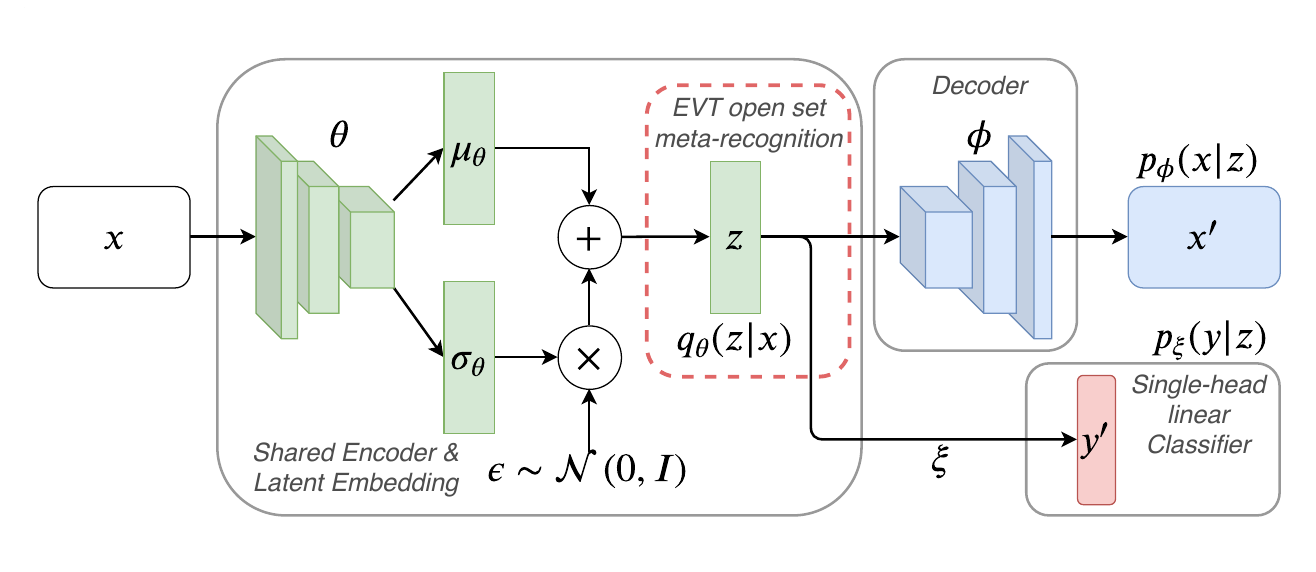
\includegraphics[width=.9\textwidth]{../model.png}
  \caption{Joint continual learning model consisting of a
  shared probabilistic encoder $q_{\theta} (z|x)$, probabilistic decoder
  $p_{\phi} (x, z)$ and probabilistic classifier $p_{xi} (y, z)$. For open set
  recognition and generative replay with outlier rejection, EVT
  based bounds on the basis of the approximate posterior are
  established.}
\end{figure}




This is particularly important to understand. Now, we have two joint probabilistic distributions consisting of three separate distributions, $~x,~y,$ and $z$. Out of the three separate distributions, two are known, $x$ and $y$ which, represent the training set input and ground truth labels. Variational inference methods takes advantage such problem setting by assuming that a joint probability
distribution of a large-enough sample set, 1) follow the same or very similar distribution of the population. 2) The non-normalized sample distribution is always smaller than the population distribution. 3) And the sample distribution is directly proportional and representative of the population distribution. On a side note, estimating the population distribution from a sample distribution through iterative means is referred to as KL-divergence and is used when deploying variational inference methods. Moreover, variational inference decomposes complex distributions into individually recognizable distributions, $z$ latent space variable vector. Thus, we can use a variational inference based auto-encoders to approximate the aggregate posterior as the following, \\
\begin{equation}
q_{\theta, t}(z) = \mathbb{E}_{p_{\tilde{D}_t} (\tilde{x})} [q_{\theta, t}(z|\tilde{x})] \\
\thickapprox \frac{1}{\tilde{N}_{t}}\sum_{n = 1}^{\tilde{N}_{t}} q_{\theta, t} (z|\tilde{x}^{(n)})
\end{equation}

%\newpage
Figure 2 depicts latent space variable projections onto $z_1 \times z_2$ phase plane.

\begin{figure}[h]
  \centering
  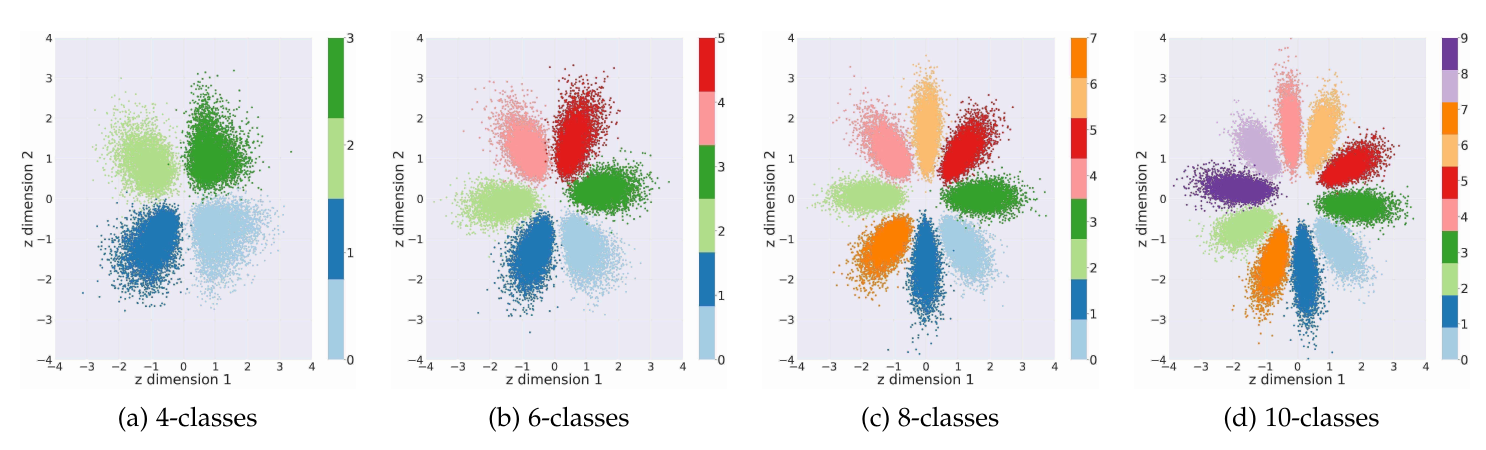
\includegraphics[width=.9\textwidth]{../z_phase.png}
  \caption{2-D latent space visualization for continually learned MNIST.}
\end{figure}

The following figures depict increased performance after rejecting outliers.

\begin{figure}[h]
  \centering
  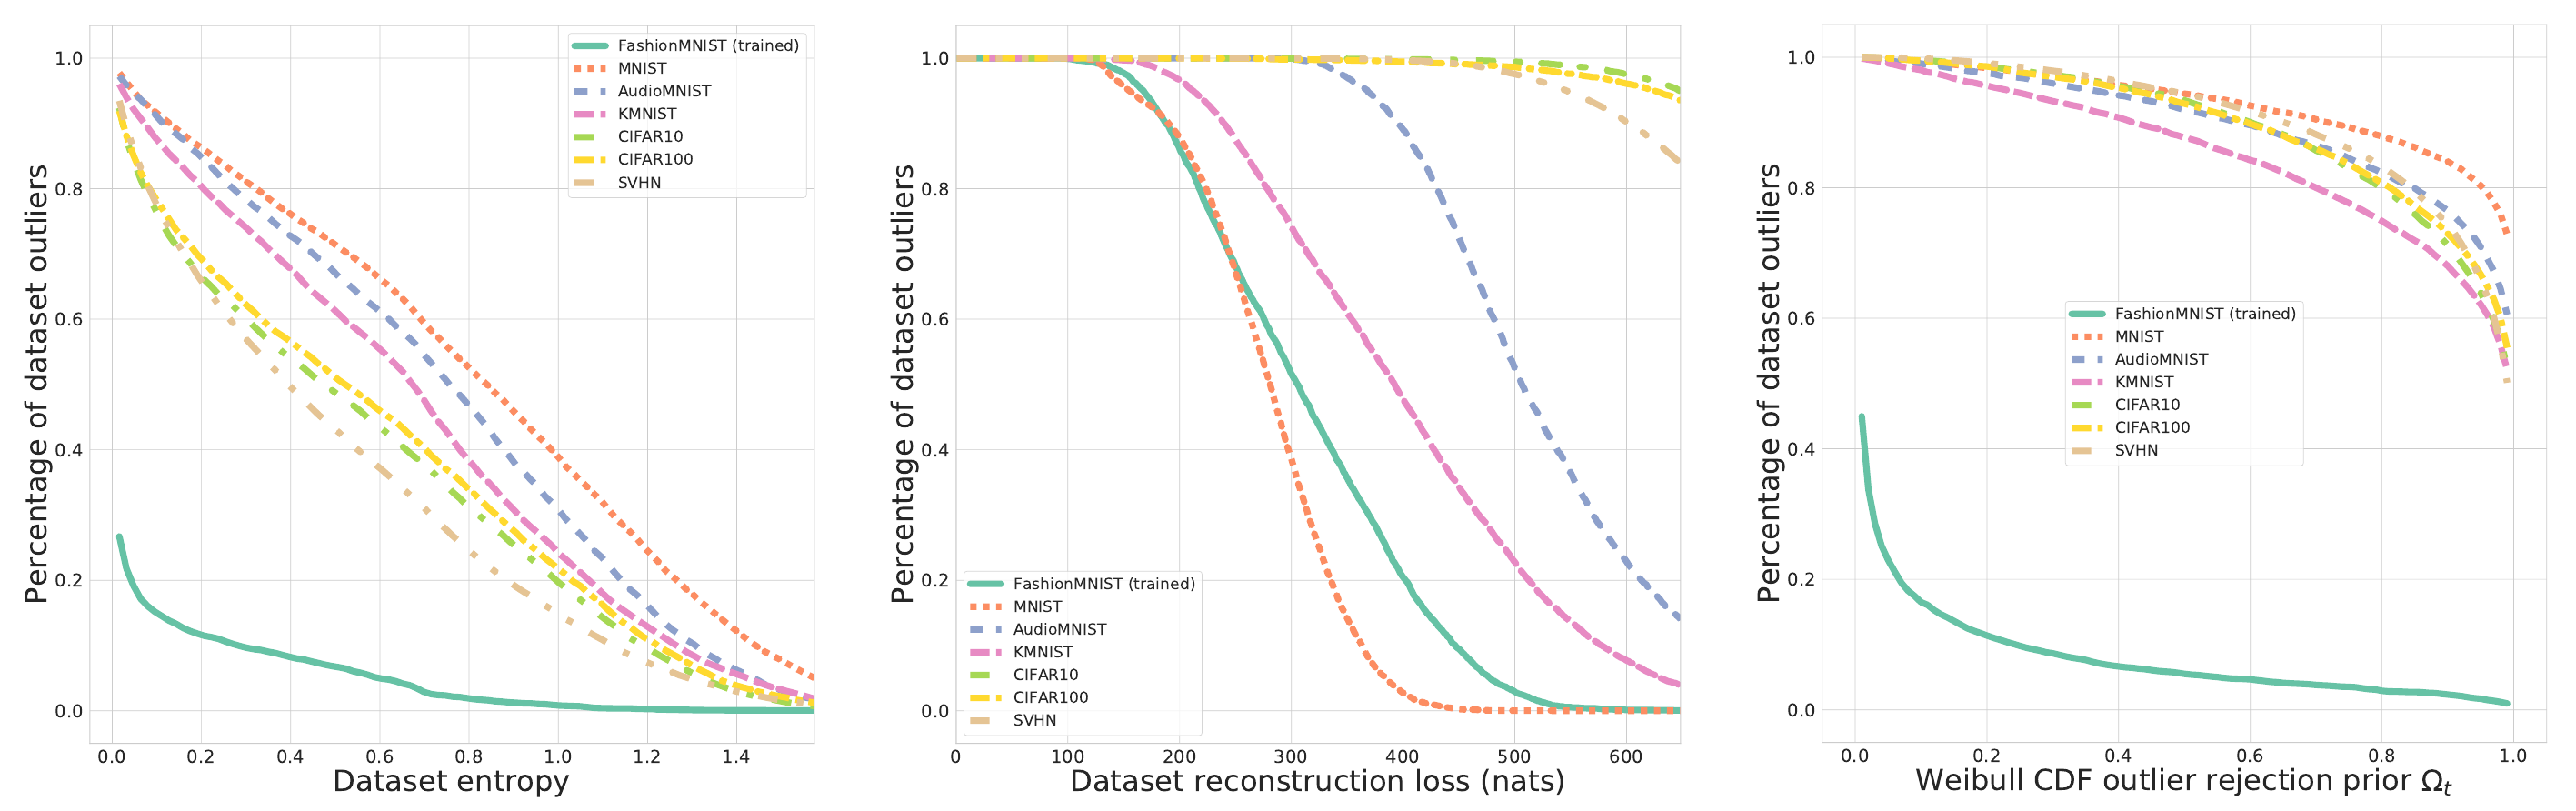
\includegraphics[width=0.8\textwidth]{../outlier.png}
  \caption{Trained Fashion MNIST OCDVAE evaluated on unknown datasets. All metrics are averaged over 100 approximate posterior samples per data point. (Left) Classifier entropy values are insufficient to separate most of unknown from the known task’s test data. (Center) Reconstruction loss allows for a partial distinction. (Right) Our posterior based open set recognition considers the large majority of unknown data as statistical outliers across a wide range of rejection priors $\Omega_t$ .
  }
\end{figure}

%Sets the bibliography style to UNSRT and import the
\newpage
\bibliography{ref}
\bibliographystyle{ieeetr}

\end{document}
